\documentclass[14pt]{extbook}
\usepackage{multicol, enumerate, enumitem, hyperref, color, soul, setspace, parskip, fancyhdr} %General Packages
\usepackage{amssymb, amsthm, amsmath, latexsym, units, mathtools} %Math Packages
\everymath{\displaystyle} %All math in Display Style
% Packages with additional options
\usepackage[headsep=0.5cm,headheight=12pt, left=1 in,right= 1 in,top= 1 in,bottom= 1 in]{geometry}
\usepackage[usenames,dvipsnames]{xcolor}
\usepackage{dashrule}  % Package to use the command below to create lines between items
\newcommand{\litem}[1]{\item#1\hspace*{-1cm}\rule{\textwidth}{0.4pt}}
\pagestyle{fancy}
\lhead{Module5}
\chead{}
\rhead{Version ALL}
\lfoot{7211-6887}
\cfoot{}
\rfoot{test}
\begin{document}

\begin{enumerate}
\item{
What is the domain of the function below?\[ f(x) = \sqrt[5]{4 x + 8} \]} \newpage
\item{
Solve the radical equation below.\[ \sqrt{16 x^2 + 25} - \sqrt{-50 x} = 0 \]} \newpage
\item{
Solve the radical equation below.\[ \sqrt{-2 x - 7} - \sqrt{6 x - 6} = 0 \]} \newpage
\item{
Write the equation of the function graphed below.
\begin{center}
    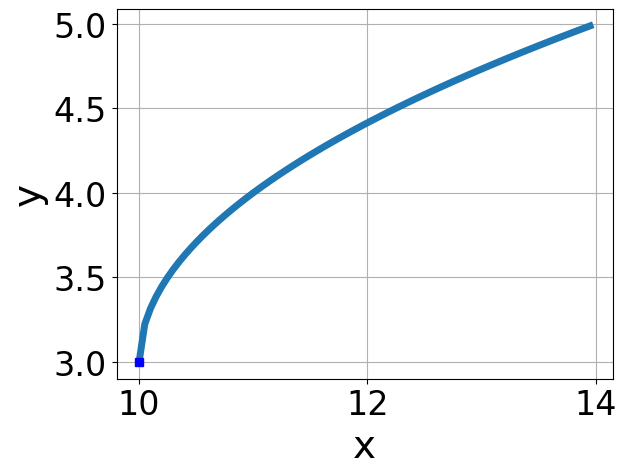
\includegraphics[width=0.5\textwidth]{../Figures/radicalGraphToEquationA.png}
\end{center}
} \newpage
\item{
Sketch a graph of the equation below.\[ f(x) = - \sqrt{x + 8} - 3 \]} \newpage
\item{
What is the domain of the function below?\[ f(x) = \sqrt[8]{-9 x + 7} \]} \newpage
\item{
Sketch a graph of the equation below.\[ f(x) = \sqrt{x - 6} + 3 \]} \newpage
\item{
Solve the radical equation below.\[ \sqrt{4 x + 2} - \sqrt{-9 x - 3} = 0 \]} \newpage
\item{
Solve the radical equation below.\[ \sqrt{35 x^2 + 8} - \sqrt{38 x} = 0 \]} \newpage
\item{
Write the equation of the function graphed below.
\begin{center}
    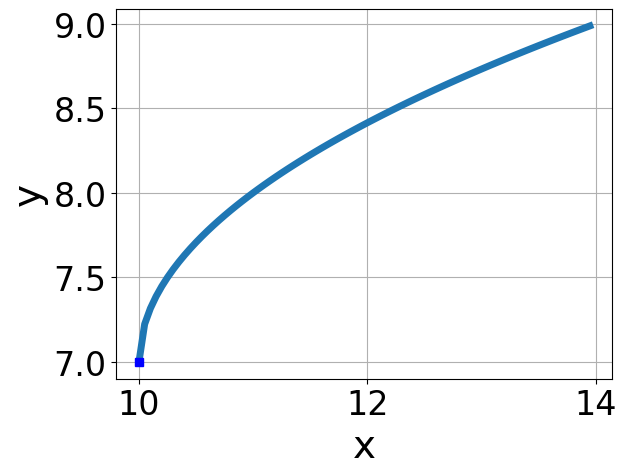
\includegraphics[width=0.5\textwidth]{../Figures/radicalGraphToEquationCopyA.png}
\end{center}
} \newpage
\item{
What is the domain of the function below?\[ f(x) = \sqrt[3]{-9 x - 3} \]} \newpage
\item{
Solve the radical equation below.\[ \sqrt{72 x^2 + 45} - \sqrt{121 x} = 0 \]} \newpage
\item{
Solve the radical equation below.\[ \sqrt{-7 x - 6} - \sqrt{-9 x - 7} = 0 \]} \newpage
\item{
Write the equation of the function graphed below.
\begin{center}
    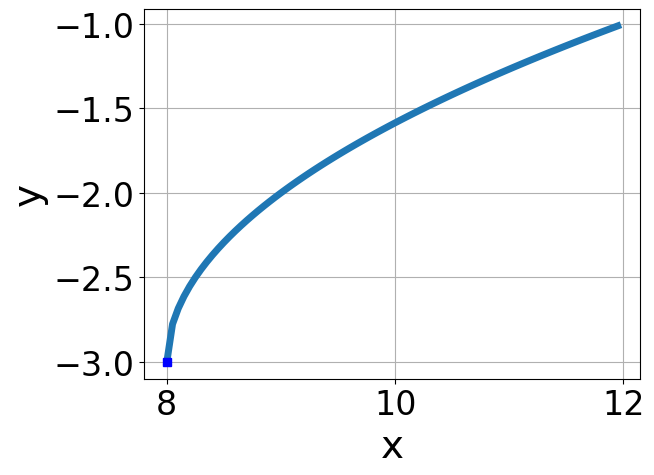
\includegraphics[width=0.5\textwidth]{../Figures/radicalGraphToEquationB.png}
\end{center}
} \newpage
\item{
Sketch a graph of the equation below.\[ f(x) = \sqrt[3]{x + 12} - 6 \]} \newpage
\item{
What is the domain of the function below?\[ f(x) = \sqrt[3]{5 x + 9} \]} \newpage
\item{
Sketch a graph of the equation below.\[ f(x) = \sqrt[3]{x - 8} - 4 \]} \newpage
\item{
Solve the radical equation below.\[ \sqrt{7 x - 4} - \sqrt{-4 x + 7} = 0 \]} \newpage
\item{
Solve the radical equation below.\[ \sqrt{24 x^2 - 10} - \sqrt{1 x} = 0 \]} \newpage
\item{
Write the equation of the function graphed below.
\begin{center}
    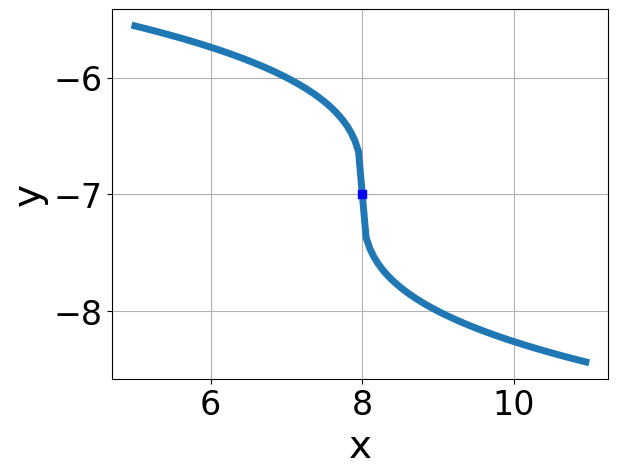
\includegraphics[width=0.5\textwidth]{../Figures/radicalGraphToEquationCopyB.png}
\end{center}
} \newpage
\item{
What is the domain of the function below?\[ f(x) = \sqrt[6]{6 x - 4} \]} \newpage
\item{
Solve the radical equation below.\[ \sqrt{49 x^2 + 30} - \sqrt{-77 x} = 0 \]} \newpage
\item{
Solve the radical equation below.\[ \sqrt{-5 x + 6} - \sqrt{-9 x + 7} = 0 \]} \newpage
\item{
Write the equation of the function graphed below.
\begin{center}
    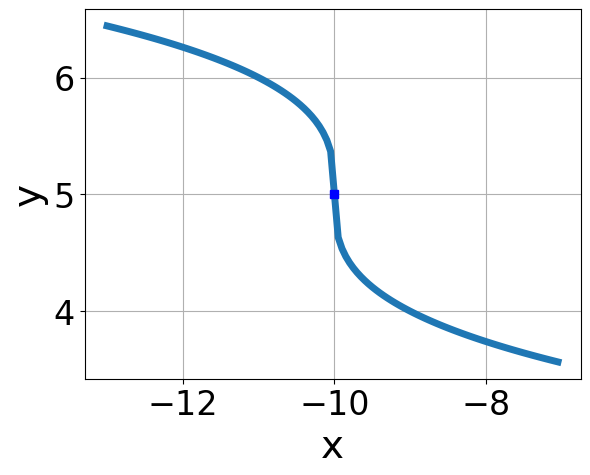
\includegraphics[width=0.5\textwidth]{../Figures/radicalGraphToEquationC.png}
\end{center}
} \newpage
\item{
Sketch a graph of the equation below.\[ f(x) = - \sqrt[3]{x - 10} + 4 \]} \newpage
\item{
What is the domain of the function below?\[ f(x) = \sqrt[8]{-4 x + 6} \]} \newpage
\item{
Sketch a graph of the equation below.\[ f(x) = - \sqrt[3]{x + 6} + 6 \]} \newpage
\item{
Solve the radical equation below.\[ \sqrt{6 x - 8} - \sqrt{-8 x + 2} = 0 \]} \newpage
\item{
Solve the radical equation below.\[ \sqrt{36 x^2 - 15} - \sqrt{-12 x} = 0 \]} \newpage
\item{
Write the equation of the function graphed below.
\begin{center}
    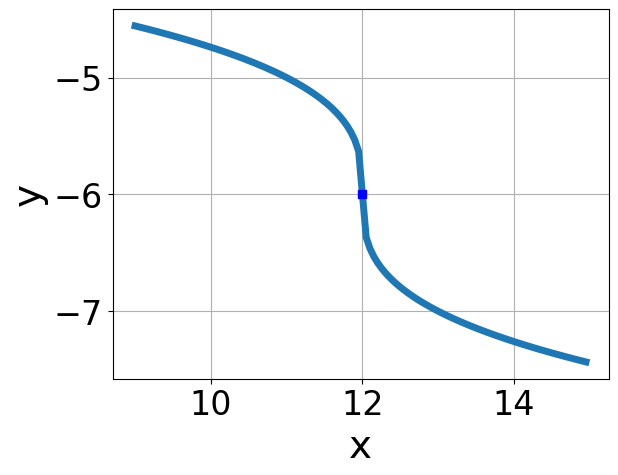
\includegraphics[width=0.5\textwidth]{../Figures/radicalGraphToEquationCopyC.png}
\end{center}
} \newpage
\end{enumerate}

\end{document}